\documentclass[10pt]{article}

\usepackage{fullpage}
\usepackage{longtable}
\usepackage[pdftex]{graphicx}
\DeclareGraphicsExtensions{.pdf,.jpg}

% no numbers, etc
\pagestyle{empty}

\begin{document}

{\bf Homework 3} \hfill {\raggedleft Thomas Torsney-Weir}

%Each homework problem goes here
\begin{enumerate}
\item % FOL chaining
  \begin{enumerate}
  \item % KB
    \begin{enumerate}
    \item Emulator(EMULATOR1)
    \item Programmer(SuperProgrammer)
    \item Writes(SuperProgrammer, EMULATOR1)
    \item $\forall x,y,z$ Programmer($x$) $\land$ Emulator($z$) $\land$ Provides($x$,$y$,$z$) $\Rightarrow$ Criminal($x$)
    \item $\forall x$ Friend($x$) $\Rightarrow$ $\neg$ Owns(GameX, $x$)
    \item $\forall x$ Friend($x$) $\Rightarrow$ Owns(EMULATOR1, $x$)
    \item $\exists y$ $\forall x, z$ Game($y$) $\land$ Emulator($x$) 
                          $\land$ Owns($x$, $z$) $\Rightarrow$ Plays($z$,$y$)
    \item $\exists y$ $\forall z$ Game($y$) $\land$ Owns(GameX, $z$) 
                          $\Rightarrow$ Plays($z$,$y$)
    \item $\forall x,y,z$ Provides($x$, $y$, $z$) $\Rightarrow$ Owns($y$,$z$)
    \item $\forall x,z$ Writes($x$,$z$) $\Rightarrow$ 
            $\exists y$ Provides($x$,$y$,$z$)
    \end{enumerate}
  \item % forward chaining
    Existential qualifiers are Skolemized and universal qualifiers are removed

    \begin{enumerate}
    \item Try Emulator(EMULATOR1) and Programmer(SuperProgrammer).  Does
          not unify.
    \item Try Emulator(EMULATOR1) and Writes(SuperProgrammer, EMULATOR1).  Does
          not unify.
    \item Try Emulator(EMULATOR1) and 
        Programmer($x$) $\land$ Emulator($z$) $\land$ \\
            Provides($x$,$y$,$z$) $\Rightarrow$ Criminal($x$). With 
        $\theta = \{z$/EMULATOR1$\}$
        yields \\
        Programmer($x$) $\land$ Emulator(EMULATOR1) $\land$ \\
            Provides($x$,$y$,EMULATOR1) $\Rightarrow$ Criminal($x$). Add to KB.
    \item Try Emulator(EMULATOR1) and 
          Friend($x$) $\Rightarrow$ $\neg$ Owns(GameX, $x$).  Does not unify.
    \item Try Emulator(EMULATOR1) and 
          Friend($x$) $\Rightarrow$ Owns(EMULATOR1, $x$). Does not unify.
    \item Try Emulator(EMULATOR1) and 
          Game(G1) $\land$ Emulator($x$) $\land$ 
            Owns($x$, $z$) $\Rightarrow$ Plays($z$,G1($x$,$z$)). With
          $\theta = \{x$/EMULATOR1$\}$ yields
          Game(G1) $\land$ Emulator(EMULATOR1) $\land$ \\
            Owns(EMULATOR1, $z$) $\Rightarrow$ Plays($z$,G1(EMULATOR1,$z$)).
          Add to KB.
    \item Try Emulator(EMULATOR1) and Game(G2($z$)) $\land$ Owns(GameX, $z$) 
            $\Rightarrow$ Plays($z$,G2($z$)). Does not unify.
    \item Try Emulator(EMULATOR1) and 
            Provides($x$, $y$, $z$) $\Rightarrow$ Owns($y$,$z$). Does not unify.
    \item Try Emulator(EMULATOR1) and 
          Writes($x$,$z$) $\Rightarrow$ Provides($x$,Y($x$,$z$),$z$).  
          Does not unify.
    \item Try Programmer(SuperProgrammer) and 
          Writes(SuperProgrammer, EMULATOR1).  Does not unify.
    \item Try Programmer(SuperProgrammer) and 
          Friend($x$) $\Rightarrow$ $\neg$ Owns(GameX, $x$).  Does not unify.
    \item Try Programmer(SuperProgrammer) and 
          Friend($x$) $\Rightarrow$ Owns(EMULATOR1, $x$). Does not unify.
    \item Try Programmer(SuperProgrammers) and 
          Game(G2($z$)) $\land$ Owns(GameX, $z$) 
            $\Rightarrow$ Plays($z$,G2($z$)). Does not unify.
    \item Try Programmer(SuperProgrammer) and 
            Provides($x$, $y$, $z$) $\Rightarrow$ Owns($y$,$z$). Does not unify.
    \item Try Programmer(SuperProgrammer) and 
          Writes($x$,$z$) $\Rightarrow$ Provides($x$,Y($x$,$z$),$z$).  
          Does not unify.
    \item Try Programmer(SuperProgrammer) and 
          Programmer($x$) $\land$ Emulator(EMULATOR1) $\land$ \\
            Provides($x$,$y$,EMULATOR1) $\Rightarrow$ Criminal($x$). With
          $\theta = \{x$/SuperProgrammer$\}$ yields \\
          Programmer(SuperProgrammer) $\land$ Emulator(EMULATOR1) $\land$ \\
            Provides(SuperProgrammer,$y$,EMULATOR1) $\Rightarrow$ 
            Criminal(SuperProgrammer). Add to KB.
    \item Try Programmer(SuperProgrammer) and 
          Game(G1) $\land$ Emulator(EMULATOR1) $\land$ \\
            Owns(EMULATOR1, $z$) $\Rightarrow$ Plays($z$,G1(EMULATOR1,$z$)).
          Does not unify.
    \item Try Writes(SuperProgrammer,EMULATOR1) and 
          Friend($x$) $\Rightarrow$ $\neg$ Owns(GameX, $x$).  Does not unify.
    \item Try Writes(SuperProgrammer,EMULATOR1) and 
          Friend($x$) $\Rightarrow$ Owns(EMULATOR1, $x$). Does not unify.
    \item Try Writes(SuperProgrammer,EMULATOR1) and 
          Game(G2($z$)) $\land$ Owns(GameX, $z$) \\
            $\Rightarrow$ Plays($z$,G2($z$)). Does not unify.
    \item Try Writes(SuperProgrammer,EMULATOR1) and 
            Provides($x$, $y$, $z$) $\Rightarrow$ Owns($y$,$z$). Does not unify.
    \item Try Writes(SuperProgrammer,EMULATOR1) and 
          Writes($x$,$z$) $\Rightarrow$ Provides($x$,Y($x$,$z$),$z$).  
          With $\theta = \{x$/SuperProgrammer, $z$/EMULATOR1$\}$ yields
          Writes(SuperProgrammer,EMULATOR1) $\Rightarrow$ 
             Provides(SuperProgrammer,Y(SuperProgrammer,EMULATOR1),EMULATOR1).
          Premise satisfied, chain conclusion.
    \item Try Provides(SuperProgrammer,Y(SuperProgrammer,EMULATOR1),EMULATOR1) 
          and \\
          Writes(SuperProgrammer, EMULATOR1).  Does not unify.
    \item Try Provides(SuperProgrammer,Y(SuperProgrammer,EMULATOR1),EMULATOR1) and \\
          Friend($x$) $\Rightarrow$ $\neg$ Owns(GameX, $x$).  Does not unify.
    \item Try Provides(SuperProgrammer,Y(SuperProgrammer,EMULATOR1),EMULATOR1) and \\
          Friend($x$) $\Rightarrow$ Owns(EMULATOR1, $x$). Does not unify.
    \item Try Provides(SuperProgrammer,Y(SuperProgrammer,EMULATOR1),EMULATOR1) and \\
          Game(G2($z$)) $\land$ Owns(GameX, $z$) 
            $\Rightarrow$ Plays($z$,G2($z$)). Does not unify.
    \item Try Provides(SuperProgrammer,Y(SuperProgrammer,EMULATOR1),EMULATOR1) 
          and \\
          Writes($x$,$z$) $\Rightarrow$ Provides($x$,Y($x$,$z$),$z$).  
          Does not unify.
    \item Try Provides(SuperProgrammer,Y(SuperProgrammer,EMULATOR1),EMULATOR1) 
          and \\
          Programmer($x$) $\land$ Emulator(EMULATOR1) $\land$ 
            Provides($x$,$y$,EMULATOR1) $\Rightarrow$ Criminal($x$). With
          $\theta = \{x$/SuperProgrammer$,$y$/Y(SuperProgrammer,EMULATOR1)\}$ 
          yields \\
          Programmer(SuperProgrammer) $\land$ Emulator(EMULATOR1) $\land$ \\
            Provides(SuperProgrammer,Y(SuperProgrammer,EMULATOR1),EMULATOR1) \\
            $\Rightarrow$ Criminal(SuperProgrammer). Which is the conclusion
            so we're done.
    \end{enumerate}
  \item % backward chaining
    \begin{enumerate}
    \item Goal is Criminal(SuperProgrammer).  Use rule
          Programmer($x$) $\land$ Emulator($z$) $\land$ \\
              Provides($x$,$y$,$z$) $\Rightarrow$ Criminal($x$).
          New goals are: Programmer(SuperProgrammer), Emulator($z$), \\
          Provides(SuperProgrammer,$y$,$z$).
    \item Goal is Programmer(SuperProgrammer).  This is in KB.
    \item Goal is Emulator($z$).  Use rule Emulator(EMULATOR1).
    \item Goal is Provides(SuperProgrammer,$y$, EMULATOR1).  Use
          rule \\
          Writes($x$,$z$) $\Rightarrow$ Provides($x$,Y($x$,$z$),$z$).
          New goal is: Writes(SuperProgrammer, EMULATOR1).
    \item Goal is Writes(SuperProgrammer, EMULATOR1).  This is in KB.
    \end{enumerate}
  \end{enumerate}
\item % FOL Resolution
  Trying to prove $\exists x$ Rel($x$, MrX, Me).
  The relationships between constants:
  \begin{itemize}
  \item $FatherMe \equiv Rel(Father, FatherMe, Me)$
  \item $Male(MrX)$
  \item $FatherX \equiv Rel(Father, FatherX, MrX)$
  \end{itemize}
  We also need to define that I have no siblings: 
  $\forall x, \neg Rel(Sibl,Me,x)$ and one for the second part of the riddle:
  $\exists f, Rel(Father, f, MrX) \land Rel(Son, FatherMe, f)$.
  And here is a list of definitions for equality:
  \begin{itemize}
  \item $Eq(x,x)$
  \item $Eq(x,y) \Rightarrow Eq(y,x)$
  \item $Eq(x,y) \land Eq(y,z) \Rightarrow Eq(x,z)$
  \item $Eq(x,y) \Rightarrow (Rel(x,w,z) \Leftrightarrow Rel(y,w,z))$
  \item $Eq(x,y) \Rightarrow (Rel(w,x,z) \Leftrightarrow Rel(w,x,z))$
  \item $Eq(x,y) \Rightarrow (Rel(w,z,x) \Leftrightarrow Rel(w,z,y))$
  \end{itemize}
  The hypothesis is: $\exists x, Rel(x, Me, MrX)$ so we want resolve with
  $\forall x, \neg Rel(x, Mr, MrX)$.
  Here are all the rules in CNF form:
  \begin{itemize}
  \item $\neg Rel(Parent,x,y) \lor \neg Male(x) \lor Rel(Father,x,y)$
  \item $\neg Rel(Father,x,y) \lor Rel(Parent,x,y)$
  \item $\neg Rel(Father,x,y) \lor Male(x)$
  \item $\neg Rel(Son,x,y) \lor Rel(Parent,y,x)$
  \item $\neg Rel(Son,x,y) \lor Male(x)$
  \item $\neg Rel(Parent,y,x) \lor \neg Male(x) \lor Rel(Son,x,y)$
  \item $\neg Rel(Sibl,x,y) \lor Neq(x,y)$
  \item $\neg Rel(Sibl,x,y) \lor Rel(Parent,P_1,x)$
  \item $\neg Rel(Sibl,x,y) \lor Rel(Parent,P_1,y)$
  \item $\neg Neq(x,y) \lor \neg Rel(Parent,p,x) \lor 
         \neg Rel(Parent,p,y) \lor Rel(Sibl,x,y)$
  \item $\neg Rel(Father,x1,y) \lor \neg Rel(Father,x2,y) \lor Eq(x,y)$
  \item $Eq(x,y) \lor Neq(x,y)$
  \item $\neg Eq(x,y) \lor \neg Neq(x,y)$
  \item $Eq(x,x)$
  \item $\neg Eq(x,y) \lor Eq(y,x)$
  \item $\neg Eq(x,y) \lor \neg Eq(y,z) \lor Eq(x,z)$
  \item $\neg Eq(x,y) \lor \neg Rel(x,w,z) \lor Rel(y,w,z)$
  \item $\neg Eq(x,y) \lor Rel(x,w,z) \lor \neg Rel(y,w,z)$
  \item $\neg Eq(x,y) \lor \neg Rel(w,x,z) \lor Rel(w,y,z)$
  \item $\neg Eq(x,y) \lor Rel(w,x,z) \lor \neg Rel(w,y,z)$
  \item $\neg Eq(x,y) \lor \neg Rel(w,z,x) \lor Rel(w,z,y)$
  \item $\neg Eq(x,y) \lor Rel(w,z,x) \lor \neg Rel(w,z,y)$
  \item $Rel(Father, FatherMe, Me)$
  \item $Male(MrX)$
  \item $Rel(Father, FatherX, MrX)$
  \item $\neg Rel(Sibl,Me,x)$.
  \item $Rel(Father,F,MrX)$
  \item $Rel(Son,F,FatherMe)$
  \item Hypothesis: $\neg Rel(w, MrX, Me)$
  \end{itemize}
  Resolution Proof:
  \ \\
  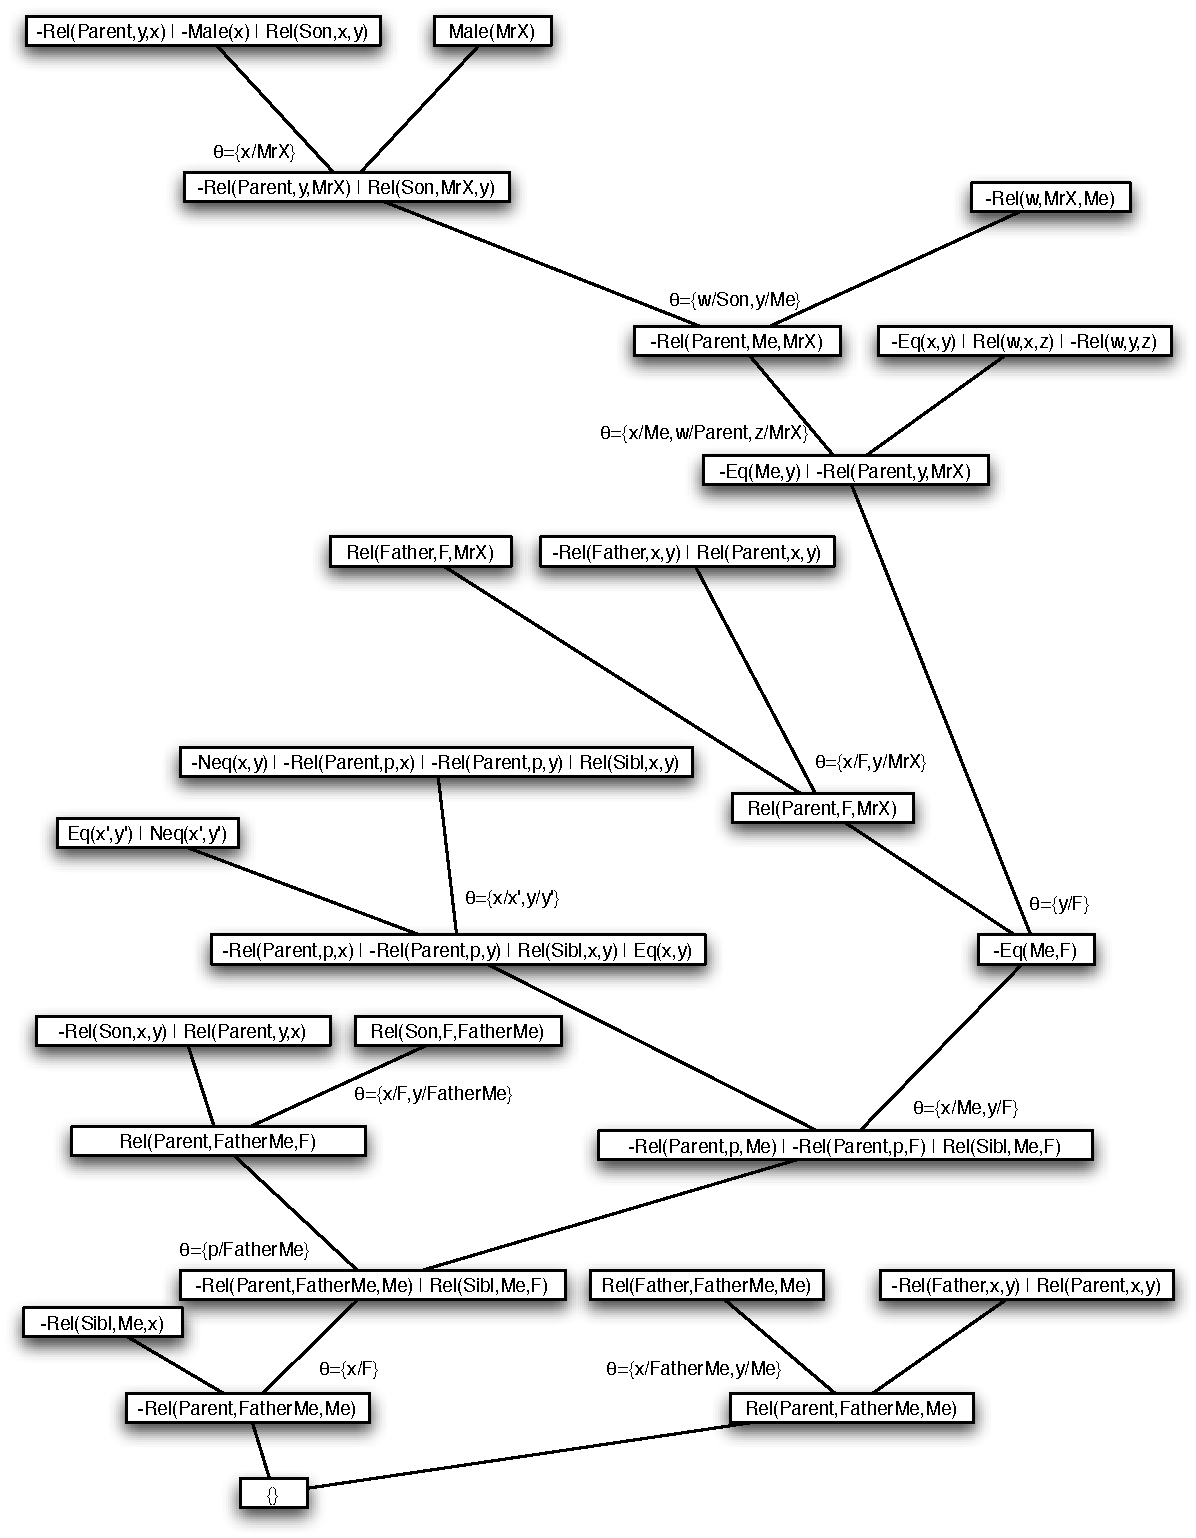
\includegraphics[width=5.5in]{3_resolution.pdf}

\item % planning
  The plan is O1 $\rightarrow$ O3 $\rightarrow$ O4 or 
  O1 $\rightarrow$ O4 $\rightarrow$ O3
  \begin{enumerate}
  \item % graphplan
    \ \\
    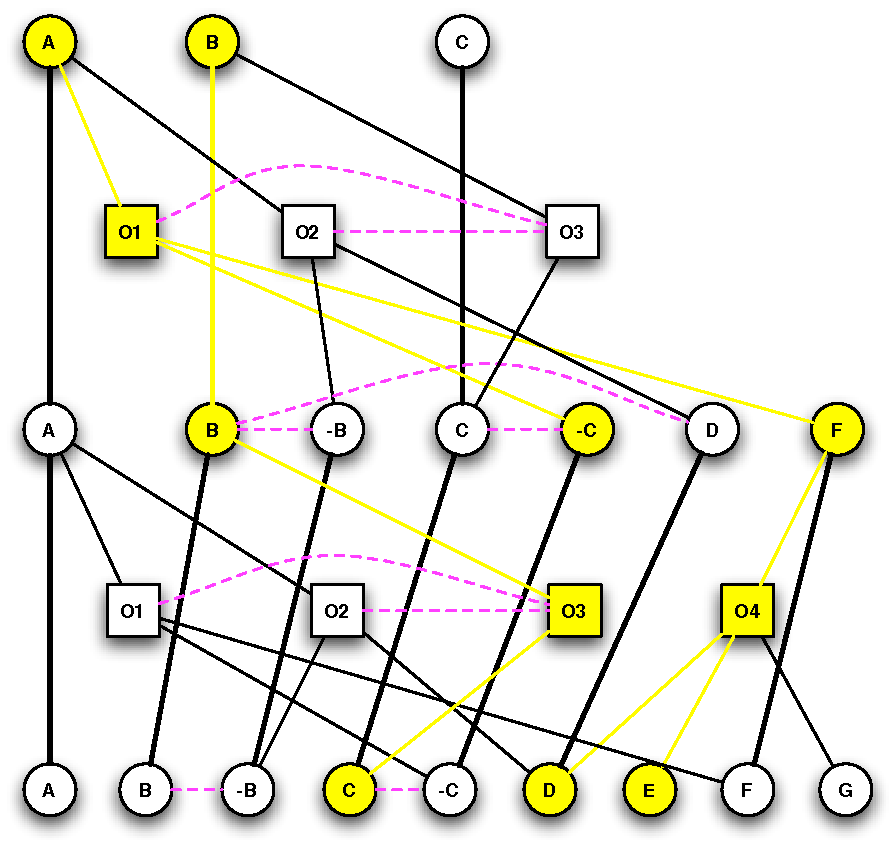
\includegraphics[width=5.5in]{4a_graphplan.pdf}
  \item % partial order
    Need C is initially satisfied by the preconditions

    \begin{tabular}{|l|l|l|l|c|c|}
    \hline
    Needs & Chosen Goal & Operator & Orderings & Causal Links \\
    \hline \hline
    D,E   &             &     & $S \prec F$  & \\
    \hline
    D,E   & E           & O4  & $S \prec F$  & $O4 \stackrel{E}{\rightarrow} F$ \\
          &             &     & $S \prec O4$ & \\
          &             &     & $O4 \prec F$ & \\
    \hline
    D,F   & D           & O4  & $S \prec F$  & $O4 \stackrel{E}{\rightarrow} F$ \\
          &             &     & $S \prec O4$ & $O4 \stackrel{D}{\rightarrow} F$ \\
          &             &     & $O4 \prec F$ & \\
    \hline
    F     &             & O1  & $S \prec F$  & $O4 \stackrel{E}{\rightarrow} F$ \\
          &             &     & $S \prec O4$ & $O4 \stackrel{D}{\rightarrow} F$ \\
          &             &     & $O4 \prec F$ & $O1 \stackrel{F}{\rightarrow} O4$ \\
          &             &     & $S \prec O1$ & \\
          &             &     & $O1 \prec O4$ & \\
    \hline
    C     &             & O3  & $S \prec F$  & $O4 \stackrel{E}{\rightarrow} F$ \\
          &             &     & $S \prec O4$ & $O4 \stackrel{D}{\rightarrow} F$ \\
          &             &     & $O4 \prec F$ & $O1 \stackrel{F}{\rightarrow} O4$ \\
          &             &     & $S \prec O1$ & $O3 \stackrel{C}{\rightarrow} F$ \\
          &             &     & $O1 \prec O4$ & \\
          &             &     & $S \prec O3$  & \\
          &             &     & $O3 \prec F$  & \\
          &             &     & $O1 \prec O3$  & \\
    \hline
    \end{tabular}
  \end{enumerate}
\item % STRIPS
  Actions:
  \begin{itemize}
  \item Op(Action: $Go(y)$, 
           Precond: $At(Shakey,x) \land In(x,r) \land In(y,r) \land Room(r)$, 
           Effect: $At(Shakey,y) \land \neg At(Shakey,x)$)
  \item Op(Action: $Push(b,x,y)$,
           Precond: $At(Shakey,x) \land In(x,r) \land In(y,r) \land 
                     Pushable(b) \land At(b,x) \land Room(r)$, 
           Effect: $At(Shakey,y) \land At(b,y) \land 
                    \neg At(Shakey,x) \land \neg At(b,y)$)
  \item Op(Action: $Climb(b)$,
           Precond: $On(Shakey,Floor) \land At(Shakey,x) \land 
                     At(b,x) \land Climbable(b)$,
           Effect: $On(Shakey,b) \land \neg On(Shakey,Floor)$)
  \item Op(Action: $Down(b)$,
           Precond: $On(Shakey,b) \land At(b,x) \land Climbable(b)$,
           Effect: $On(Shakey,Floor) \land \neg On(Shakey,b)$)
  \item Op(Action: $TurnOn(ls)$,
           Precond: $On(Shakey,b) \land At(b,x) \land At(ls,x) \land
                     In(ls,r) \land LightOff(r)$,
           Effect: $LightOn(r) \land \neg LightOff(r)$)
  \item Op(Action: $TurnOff(ls)$,
           Precond: $On(Shakey,b) \land At(b,x) \land At(ls,x) \land
                     In(ls,r) \land LightOn(r)$,
           Effect: $LightOff(r) \land \neg LightOn(r)$)
  \end{itemize}

  Initial State: 
  \begin{eqnarray*}
  & & At(B1,a) \land At(B2,b) \land At(B3,c) \land At(B4,d) \land In(a,R1) \land
      In(b,R2) \land In(c,R3) \land In(d,R4) \land \\
  & & LightOn(R1) \land LightOn(R2) \land LightOn(R3) \land LightOn(R4) \land 
      In(Ls1,R1) \land In(Ls2,R2) \land \\
  & & In(Ls3,R3) \land In(Ls4,R4) \land In(D1,R1) \land
      In(D1,Corridor) \land In(D2,R2) \land In(D2,Corridor) \land \\
  & & In(D3,R3) \land In(D3,Corridor) \land In(D4,R4) \land 
      In(D4,Corridor) \land At(D1,z1) \land At(D2,z2) \land \\
  & & At(D3,z3) \land At(D4,z4) \land Pushable(B1) \land 
      Pushable(B2) \land Pushable(B3) \land Pushable(B4) \land \\
  & & Climbable(B1) \land Climbable(B2) \land Climbable(B3) \land 
      Climbable(B4) \land At(Shakey,x) \land \\
  & & In(R3,x) \land On(Shakey,Floor)
  \end{eqnarray*}

  Plan: $Go(z3)$, $Go(z1)$, $Go(b)$, $Push(B1,b,z1)$, $Push(B1,z1,z2)$
\end{enumerate}

\end{document}

